\documentclass{standalone}
\usepackage{tikz}
\usepackage{ctex,siunitx}
\usepackage{tkz-euclide}
\usepackage{amsmath}
\usetikzlibrary{patterns, calc}
\usetikzlibrary {decorations.pathmorphing, decorations.pathreplacing, decorations.shapes,}
\begin{document}
\small
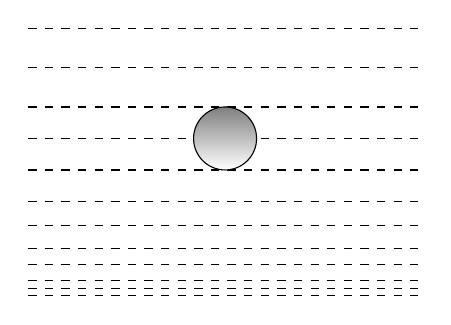
\begin{tikzpicture}[>=stealth,scale=1]
  \foreach \x in {0,0.1,0.2,0.4,.6,.9,1.2,1.6,2,2.4,2.9,3.4}
  {
    \draw [dashed](0,\x)--(5,\x);
  }
  \draw [shade] (2.5,2) circle (4mm);
\end{tikzpicture}
\end{document}